\documentclass[uplatex]{jsarticle}

\usepackage{amsmath}
\usepackage[dvipdfmx]{graphicx}

\setcounter{tocdepth}{3}
\usepackage{float}
\usepackage{moreverb}
\usepackage{lscape}
%\pagestyle{empty}
%\usepackage{wrapfig}
%\usepackage{url}
%\usepackage{EasyLayout}


\usepackage{ascmac}
%\usepackage{fancybx}

%\pagestyle{myheadings}


\begin{document}


\title{6回目の課題}
\author{25G1065 塩澤匠生}
%\date{2015年11月13日}
\maketitle


\section{はじめに}

\section{手法}

\subsection{方程式の説明}

今回は(\ref{eq:f1}) 式を用いて、二分法とニュートン法の収束するまでの試行回数を比較する。
\begin{equation}\label{eq:f1}
    f(x) = \cos x - x^2 = 0
\end{equation}
\begin{figure}[H]
    \centering
    % \hspace{-4cm} % 左にずらす
    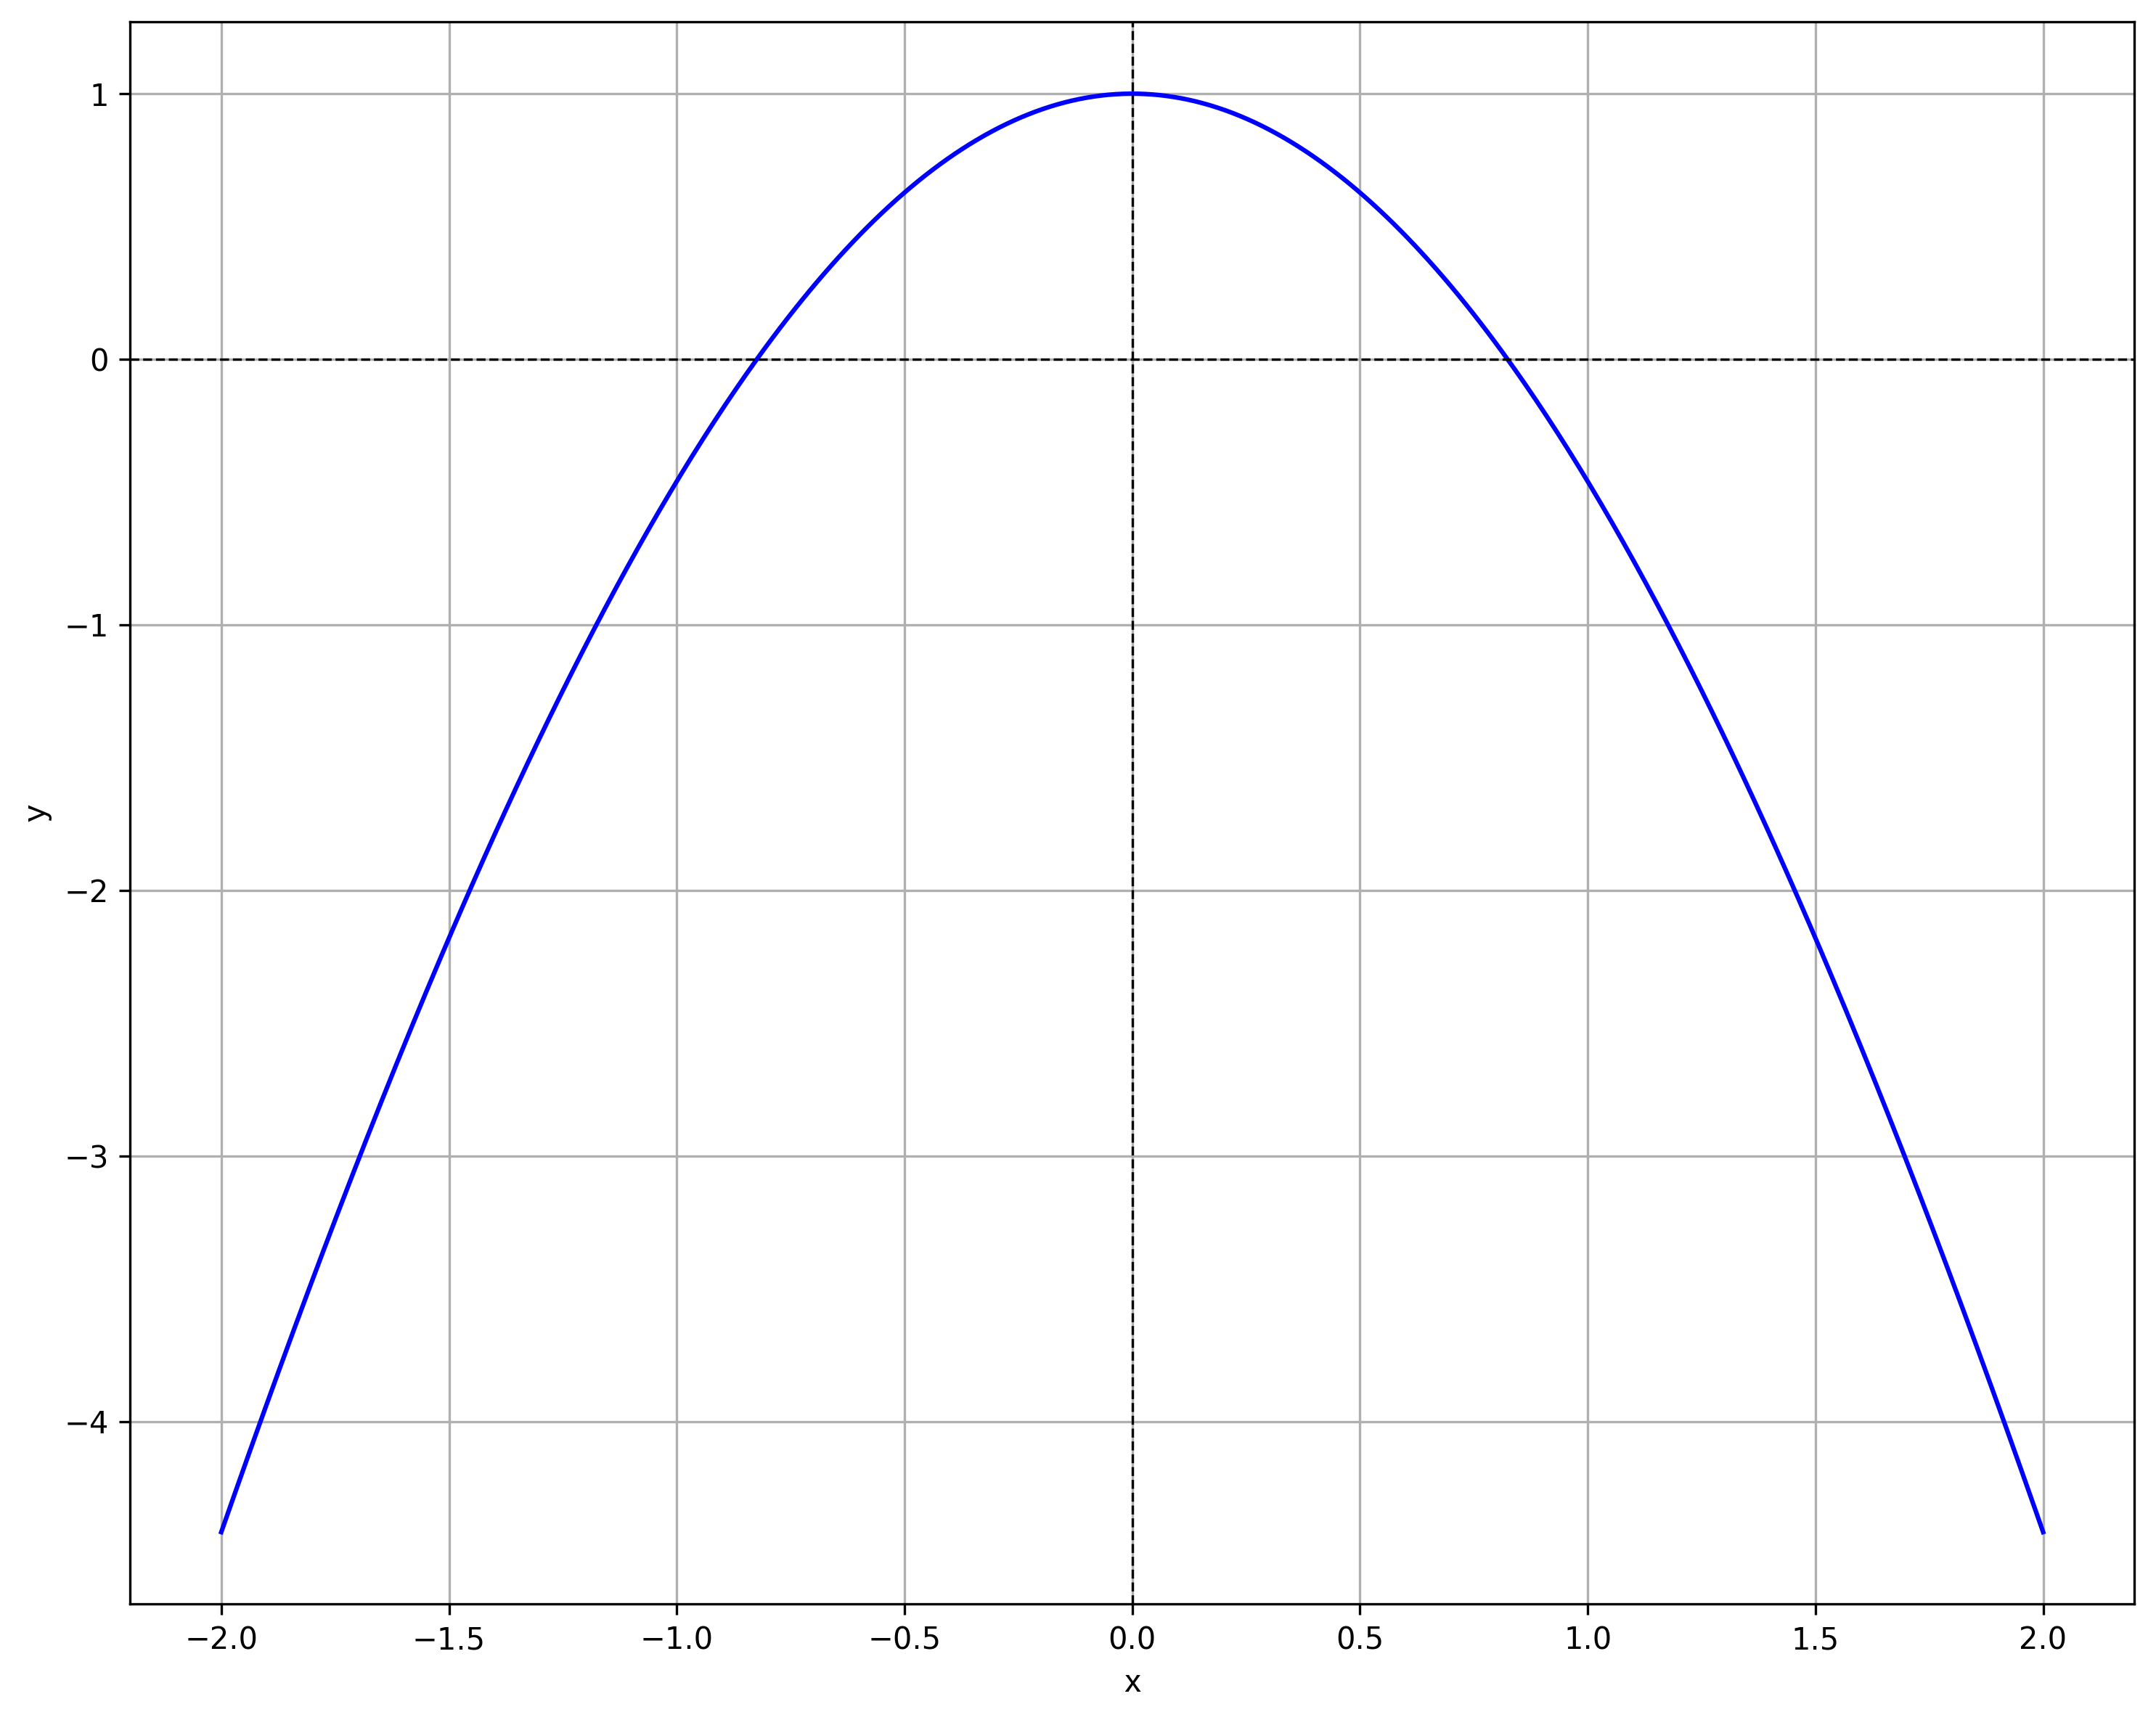
\includegraphics[width=0.8\textwidth]{graph/f1.png}
    \caption{$f(x) = \cos x - x^2$ のグラフ}
    \label{fig:f1graph}
\end{figure}

\subsection{二分法・ニュートン法の説明}

二分法\\
関数名:bisection 入力:探索範囲の下端a、上端b、許容誤差tol
処理:c=(a+b)/2を計算し、f(a)f(c)<0ならb=c, そうでなければa=cとして値を更新しながら
a-bの値が許容誤差tolを下回るまで繰り返す。
出力:反復回数、繰り返し毎の推定解、誤差。\\

ニュートン法\\
関数名:newton 入力:xnの初期値x0、許容誤差tol、最大反復回数max\_iter
処理:n=0,1,2,…に対して\( x_{n+1} = x_n - \frac{f(x_n)}{f'(x_n)} \)にする処理を
\( x_{n+1} - x_n \)が許容誤差\( \text{tol} \)を下回る、または反復回数が最大反復回数
\( \text{max\_iter} \)を上回るまで繰り返す。
出力:反復回数、繰り返し毎の推定解、誤差。



\section{結果}

\section{おわりに}


\end{document}



























